% *********************************************************************
% © 2021–2024 Jeremy Sylvestre
%
% Permission is granted to copy, distribute and/or modify this document
% under the terms of the GNU Free Documentation License, Version 1.3 or
% any later version published by the Free Software Foundation; with no
% Invariant Sections, no Front-Cover Texts, and no Back-Cover Texts. A
% copy of the license is included in the appendix entitled “GNU Free
% Documentation License” that appears in the output document of this
% PreTeXt source code. All trademarks™ are the registered® marks of
% their respective owners.
%
% *********************************************************************

\newcommand*{\xmin}{-0.5}
\newcommand*{\xmax}{5.5}
\newcommand*{\ymin}{-0.5}
\newcommand*{\ymax}{1.5}

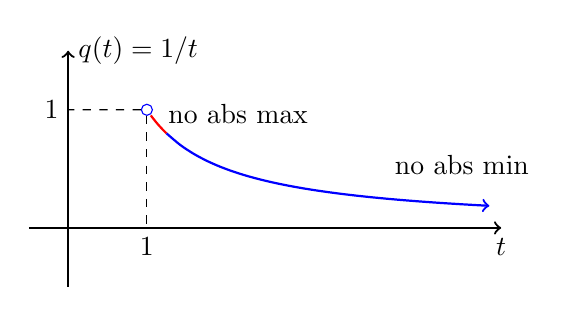
\begin{tikzpicture}
[
	closedpt/.style={circle,draw,fill,inner sep=0pt,minimum size=4pt},
	openpt/.style={circle,draw,inner sep=0pt,minimum size=4pt},
	yscale=1.5
]

	% axes
	\draw[->,thick] (\xmin,0) -- (\xmax,0) node[below] {$t$};
	\draw[->,thick] (0,\ymin) -- (0,\ymax) node[right] {$q(t) = 1/t$};

	% graph
	\draw[thick, red, domain=1.05:1.25, smooth] plot (\x,{1 / \x});
	\draw[->,thick, blue, domain=1.25:5.35, smooth] plot (\x,{1 / \x});

	\node[blue,openpt] at (1,1) (start) {};
	\draw[dashed] (start) -- (0,1) node[left] {$1$};
	\draw[dashed] (start) -- (1,0) node[below] {$1$};

	\node[above,yshift=0.25cm] at (5,0.2) {no abs min};
	\node[right,yshift=-0.05cm,xshift=0.15cm] at (1,1) {no abs max};

\end{tikzpicture}
